\documentclass[conference]{IEEEtran}
\IEEEoverridecommandlockouts

\usepackage{cite}
\usepackage{amsmath,amssymb}
\usepackage{graphicx}
\usepackage{booktabs}
\usepackage{url}
\usepackage[hidelinks]{hyperref}

\graphicspath{{../figuras/}}

% As tabelas sao geradas por paper/gerar_tabelas.py a partir do dataset.
% Nunca editar tabelas/*.tex na mao: rode o script de novo.

\begin{document}

% =====================================================================
% TITLE (5 pts)
% Alternativas consideradas (o enunciado pede que se tente mais de uma):
%   A) Exploratory Analysis of a 50,000-Patient Synthetic Diabetes Risk
%      Dataset: Strong Univariate Separability with Near-Absent
%      Multivariate Structure                                  <- segura
%   B) What Principal Component Analysis Reveals About a Synthetic
%      Dataset: Glycemic Markers Separate Diabetes Risk Classes
%      That PCA Cannot                                    <- mais forte
%   C) Fasting Glucose and HbA1c Alone Separate Diabetes Risk Classes
%      in a Synthetic 50,000-Patient Cohort
% =====================================================================
\title{Exploratory Analysis of a 50{,}000-Patient Synthetic Diabetes
Risk Dataset: Strong Univariate Separability with Near-Absent
Multivariate Structure}

% Com 4 autores o \and do IEEEtran joga todos numa linha so e as colunas
% ficam com larguras diferentes, porque os nomes tem tamanhos diferentes.
% Duas linhas de dois, em minipages de largura fixa, ficam simetricas.
% Os macros \IEEEauthorblockN/A so funcionam na estrutura propria do \author
% do IEEEtran, entao dentro da minipage usamos formatacao direta, com os
% mesmos corpos de letra que eles aplicam.
\newcommand{\autorbloco}[2]{%
  \begin{minipage}[t]{0.46\textwidth}\centering
  {\normalsize #1}\\[0.35em]
  {\small #2\\
  \textit{Dep.\ de Eng.\ de Teleinformática}\\
  \textit{Universidade Federal do Ceará}}
  \end{minipage}}

% O \author do IEEEtran ja e um ambiente tabular, entao um \\ solto abriria
% linha nova nesse tabular e quebraria a compilacao. O \parbox isola.
\author{%
\parbox{\textwidth}{\centering
\autorbloco{Ícaro Adriano}{609310}\hfill\autorbloco{Matheus Reis}{571954}\\[1.4em]
\autorbloco{Alisson Jaime}{555083}\hfill\autorbloco{Vinícius A. G. do Nascimento}{568594}}
}

\maketitle

% =====================================================================
% ABSTRACT (10 pts) -- 4 frases: objetivo, dados, metodos, resultado.
% ATENCAO: nao prometer machine learning. O trabalho e exploratorio.
% =====================================================================
\begin{abstract}
% [1] Objetivo
This work presents an exploratory analysis of a publicly available
synthetic dataset of diabetes risk, with the goal of characterising
which of its predictors carry discriminative information before any
predictive model is considered.
% [2] Dados
The dataset comprises $N = 50{,}000$ records, $D = 22$ predictors and
$L = 3$ risk classes, with a strongly imbalanced class distribution in
which the \emph{Low} class holds only $0.94\%$ of the observations.
% [3] Metodos
We combine unconditional and class-conditional univariate statistics,
pairwise Pearson correlation and a principal component analysis (PCA)
implemented from first principles, without recourse to pre-made PCA
routines.
% [4] Resultado principal
Two glycemic markers, fasting blood sugar and HbA1c, separate the risk
classes almost by themselves, yet the first two principal components
account for only $15.2\%$ of the total variance. Three independent
lines of evidence, an excess kurtosis of $-1.2$ in 19 of the 20
quantitative predictors, a median absolute pairwise correlation of
$0.003$, and an eigenvalue spectrum flat at unity, converge on the same
conclusion: the predictors were drawn independently from bounded
uniform distributions, and the only structural relationship the data
contain is the algebraic identity that defines the body mass index.
\end{abstract}

\begin{IEEEkeywords}
exploratory data analysis, principal component analysis, synthetic
data, diabetes risk, class separability
\end{IEEEkeywords}

% =====================================================================
% I. INTRODUCTION (20 pts) -- alvo: 1 pagina, 4 paragrafos.
% =====================================================================
\section{Introduction}
\label{sec:intro}

% --- P1: diabetes como problema de saude publica + deteccao precoce.
% Referencias externas entram aqui (IDF/ADA).
Diabetes mellitus is one of the largest public health burdens
worldwide \cite{idf2021}. In 2024, 589 million adults aged 20 to 79
years, one in every nine, were living with the condition, and this
figure is projected to reach 853 million by 2050, a 45\% rise against
a projected population growth of 25\%. A further 252 million adults
are estimated to be unaware that they have it. The disease accounted
for 3.4 million deaths and for at least USD 1 trillion in health
expenditure in that single year, which is what makes early detection
consequential: it opens a window for treatment and lifestyle
intervention before microvascular and cardiovascular complications
become established.

% --- P2: por que analise exploratoria antes de modelagem.
% Este paragrafo justifica a existencia do trabalho.
Fitting a classifier without a prior exploratory analysis makes it
impossible to tell whether the performance obtained reflects genuine
clinical patterns or artefacts of the data. Descriptive statistics and
linear projections expose, beforehand, redundancy among predictors,
disparities of scale, outliers and the degree of overlap between the
classes. Without that map of the underlying structure, neither the
success nor the failure of a model can be diagnosed.

% --- P3: datasets sinteticos em saude. ESTE e o paragrafo que
% diferencia o trabalho: privacidade, volume, ensino, e as limitacoes.
% Prepara a discussao dos resultados e a conclusao.
The use of synthetic datasets in health care has grown as a way of
circumventing strict patient privacy constraints, of compensating for
the scarcity of records and of enabling educational applications
\cite{synthetic2021}. That convenience, however, carries the risk that
the generating process fails to reproduce the complex physiological
interdependencies present in real clinical populations. When
multivariate relationships are not preserved, algorithms trained on
such data tend to learn mathematical artefacts rather than legitimate
biological mechanisms. It is in this context that the dataset analysed
here belongs, its origin being explicitly synthetic \cite{kaggle2024}.

% --- P4: objetivo e organizacao do artigo.
This work presents an exploratory and multivariate characterisation of
a synthetic dataset of diabetes risk, assessing its statistical
consistency and its clinical fidelity before any modelling step. We
investigate the dependencies among predictors and determine to what
extent the risk classes are structurally separable, both in the
original predictor space and under projections of maximum variance.
The remainder of this paper is organised as follows.
Section~\ref{sec:methods} describes the dataset and the analytical
methods. Section~\ref{sec:results} reports and discusses the results.
Section~\ref{sec:conclusion} concludes.

% =====================================================================
% II. METHODS (30 pts) -- alvo: 1,5 pagina.
% Regra do enunciado: TODA figura e TODA tabela citada e comentada
% no texto corrido. Nenhuma float orfa.
% =====================================================================
\section{Methods}
\label{sec:methods}

\subsection{Dataset}
\label{subsec:dataset}

% Fonte, natureza sintetica, N, D, L.
The dataset was obtained from Kaggle \cite{kaggle2024} and is
explicitly described by its authors as a large-scale \emph{synthetic}
healthcare dataset. The raw file holds 41 columns, from which we
discard \texttt{Patient\_ID}, a row identifier carrying no
physiological information, and \texttt{Diabetes\_Risk\_Score}, the
continuous score from which the categorical label is derived. This
leaves $N = 50{,}000$ observations and $D = 22$ predictors, of which 20
are quantitative and two (\texttt{Country} and \texttt{Gender}) are
categorical. The class label \texttt{Diabetes\_Risk} takes $L = 3$
values.

% Distribuicao de classes: comentar o desbalanceamento (Low < 1%).
Table~\ref{tab:classdist} reports the class distribution.
The disparity between the 36{,}593 observations of class \emph{High}
and the 470 of class \emph{Low}, a ratio of 78 to 1 and a mere
$0.94\%$ of the sample, imposes structural limits on the analysis. It
renders the class-conditional estimates of the minority class
unstable, and it would compromise the evaluation of any future
classifier, since a naive model that constantly predicts \emph{High}
would already reach $73\%$ accuracy.

\begin{table}[htbp]
\caption{Class distribution of \texttt{Diabetes\_Risk}}
\label{tab:classdist}
\centering
\begin{tabular}{lrr}
\toprule
Class & $N_l$ & Share \\
\midrule
High & 36{,}593 & 73.19\% \\
Moderate & 12{,}937 & 25.87\% \\
Low & 470 & 0.94\%
\\
\midrule
Total & 50{,}000 & 100.00\% \\
\bottomrule
\end{tabular}
\end{table}

% Valores faltantes: o padrao de exatos 1000 no painel lipidico
% e observacao propria e vale ponto.
Table~\ref{tab:missing} summarises the missing values, which affect 12
of the 20 quantitative predictors.
Four of them are missing \emph{exactly} one thousand values each, and
those four are precisely the complete lipid panel: total cholesterol,
HDL, LDL and triglycerides. A fifth column outside the quantitative
set, medication adherence, shows the same round count. Natural record
loss does not produce an identical round figure across five variables,
so the absences were evidently injected by the generator. They were
not injected by examination, however: no observation lacks all four
lipid measurements at once, and the pairwise overlap between them
ranges from 12 to 21 rows, which is what independent sampling of $2\%$
of the records would yield. In clinical practice a lipid panel is a
single blood draw and its four results go missing together; here a
fixed quota of one thousand absences was drawn column by column,
ignoring that dependency.

\begin{table}[htbp]
\caption{Missing values (only affected predictors shown)}
\label{tab:missing}
\centering
\begin{tabular}{lr}
\toprule
Predictor & Missing \\
\midrule
Weight kg & 2{,}962 \\
Height cm & 2{,}945 \\
Sleep Hours & 2{,}017 \\
Exercise Hours Per Week & 1{,}992 \\
HbA1c & 1{,}974 \\
Daily Walking Minutes & 1{,}964 \\
LDL & 1{,}000 \\
HDL & 1{,}000 \\
Total Cholesterol & 1{,}000 \\
Triglycerides & 1{,}000 \\
Blood Glucose & 959 \\
Age & 497
\\
\bottomrule
\end{tabular}
\end{table}

\subsection{Pre-processing}
\label{subsec:preproc}

% Padronizacao e dropna, com a limitacao dos 33%.
Standardising the variables to zero mean and unit variance before the
principal component analysis is mandatory, since the raw predictors
operate on widely disparate scales (mg/dL, kg, cm, years); without
that correction the variables of larger magnitude would dominate the
covariance matrix and the analysis would describe the units of
measurement rather than the intrinsic structure of the data.
Furthermore, because the covariance matrix requires complete records,
the rows holding missing values were removed. This exclusion reduced
the set from $50{,}000$ to $33{,}689$ observations, that is, $32.6\%$
of the data discarded, and it establishes a methodological limitation:
the multivariate analysis describes a complete subset and not the
entire cohort. The univariate and bivariate statistics, in contrast,
use every observation available for each predictor.

\subsection{Analytical methods}
\label{subsec:methods}

% Embasamento teorico exigido pelo enunciado. Definir cada estatistica
% e dizer o que ela informa.
For each predictor $d$ we compute the mean $\mu_d$, the standard
deviation $\sigma_d$ and the skewness $\gamma_d$,
\begin{equation}
\gamma_d = \frac{1}{N}\sum_{n=1}^{N}
\left(\frac{x_{n,d}-\mu_d}{\sigma_d}\right)^{3},
\label{eq:skew}
\end{equation}
which quantifies the imbalance between the tails of a distribution and
vanishes for any density symmetric about its mean,
together with the excess kurtosis, the analogous fourth-order moment
minus three, and their class-conditional counterparts $\mu_{d|l}$,
$\sigma_{d|l}$ and $\gamma_{d|l}$ over the $N_l$ observations of each
class $l$. Skewness vanishes for any symmetric distribution and so
cannot by itself distinguish a Gaussian from a uniform density, whereas
the excess kurtosis separates them cleanly: it is $0$ for the Gaussian
and $-6/5$ for the uniform. We therefore report both.

% Correlacao de Pearson: dizer o que capta e o que NAO capta.
Linear dependence between pairs of predictors is quantified by the
Pearson correlation coefficient
\begin{equation}
\rho_{d_i,d_j} =
\frac{\mathbb{E}\left[(X_{d_i}-\mu_{d_i})(X_{d_j}-\mu_{d_j})\right]}
{\sigma_{d_i}\sigma_{d_j}},
\label{eq:pearson}
\end{equation}
which captures linear association only. A vanishing $\rho$ does not
imply independence in general, so we treat the correlation matrix as
one piece of evidence among three rather than as a conclusion.

% Poder discriminativo: definir a metrica usada, pois nao e padrao.
To rank predictors by their ability to separate classes on their own,
we use the ratio between the range of the class-conditional means and
the unconditional standard deviation,
\begin{equation}
\delta_d = \frac{\max_l \mu_{d|l} - \min_l \mu_{d|l}}{\sigma_d},
\label{eq:discrim}
\end{equation}
so that $\delta_d$ expresses the class separation in units of the
predictor's own spread and is comparable across predictors measured in
different physical units.

% PCA implementado do zero: o enunciado EXIGE que se diga isso.
Finally, the principal component analysis was implemented from
scratch, without pre-made PCA functions or libraries, following the
standard chain \cite{jolliffe2002}: standardisation, estimation of the
covariance matrix $\mathbf{S}$, eigendecomposition
$\mathbf{S} = \mathbf{V}\boldsymbol{\Lambda}\mathbf{V}^{\top}$, and
projection of the observations onto the two eigenvectors of largest
eigenvalue. The only library routine used is the symmetric
eigensolver.

% =====================================================================
% III. RESULTS (35 pts) -- alvo: 2,5 paginas. Secao que decide a nota.
% Quatro blocos, na ordem das perguntas do enunciado.
% =====================================================================
\section{Results and Discussion}
\label{sec:results}

\subsection{Unconditional univariate analysis}
\label{subsec:uncond}

% Bloco 1. Tabela completa + histogramas.
Table~\ref{tab:uncond} reports $\mu_d$, $\sigma_d$, $\gamma_d$, the
excess kurtosis and the observed range of the 20 quantitative
predictors, and Fig.~\ref{fig:hist} shows the corresponding
histograms.

\begin{table*}[htbp]
\caption{Unconditional univariate statistics of the 20 quantitative
predictors. The excess kurtosis of a uniform distribution is $-6/5$.}
\label{tab:uncond}
\centering
\begin{tabular}{lrrrrr}
\toprule
Predictor & $\mu_d$ & $\sigma_d$ & $\gamma_d$ & Excess kurtosis & Range \\
\midrule
Age & 53.87 & 21.13 & +0.008 & -1.206 & 18.0--90.0 \\
Height cm & 170.02 & 14.46 & +0.000 & -1.207 & 145.0--195.0 \\
Weight kg & 87.46 & 24.50 & +0.004 & -1.191 & 45.0--130.0 \\
BMI & 30.92 & 10.29 & +0.432 & -0.453 & 11.9--61.7 \\
Waist Circumference cm & 99.96 & 23.09 & +0.010 & -1.191 & 60.0--140.0 \\
Blood Glucose & 159.91 & 52.04 & +0.006 & -1.212 & 70.0--250.0 \\
HbA1c & 8.49 & 2.31 & +0.002 & -1.204 & 4.5--12.5 \\
Fasting Blood Sugar & 142.61 & 44.68 & -0.001 & -1.200 & 65.0--220.0 \\
Insulin Level & 23.48 & 12.40 & +0.006 & -1.200 & 2.0--45.0 \\
Blood Pressure Systolic & 140.17 & 29.17 & -0.004 & -1.201 & 90.0--190.0 \\
Blood Pressure Diastolic & 90.04 & 17.58 & -0.010 & -1.193 & 60.0--120.0 \\
Total Cholesterol & 220.17 & 57.79 & -0.005 & -1.203 & 120.0--320.0 \\
HDL & 57.37 & 18.72 & +0.004 & -1.195 & 25.0--90.0 \\
LDL & 135.01 & 49.14 & -0.004 & -1.205 & 50.0--220.0 \\
Triglycerides & 229.54 & 98.23 & -0.000 & -1.200 & 60.0--400.0 \\
Heart Rate & 85.12 & 20.39 & -0.015 & -1.189 & 50.0--120.0 \\
Exercise Hours Per Week & 5.02 & 2.88 & -0.009 & -1.192 & 0.0--10.0 \\
Daily Walking Minutes & 89.93 & 52.03 & +0.005 & -1.206 & 0.0--180.0 \\
Sleep Hours & 6.50 & 2.03 & -0.005 & -1.210 & 3.0--10.0 \\
Daily Water Intake L & 3.00 & 1.15 & +0.003 & -1.189 & 1.0--5.0
\\
\bottomrule
\end{tabular}
\end{table*}

\begin{figure}[htbp]
\centering
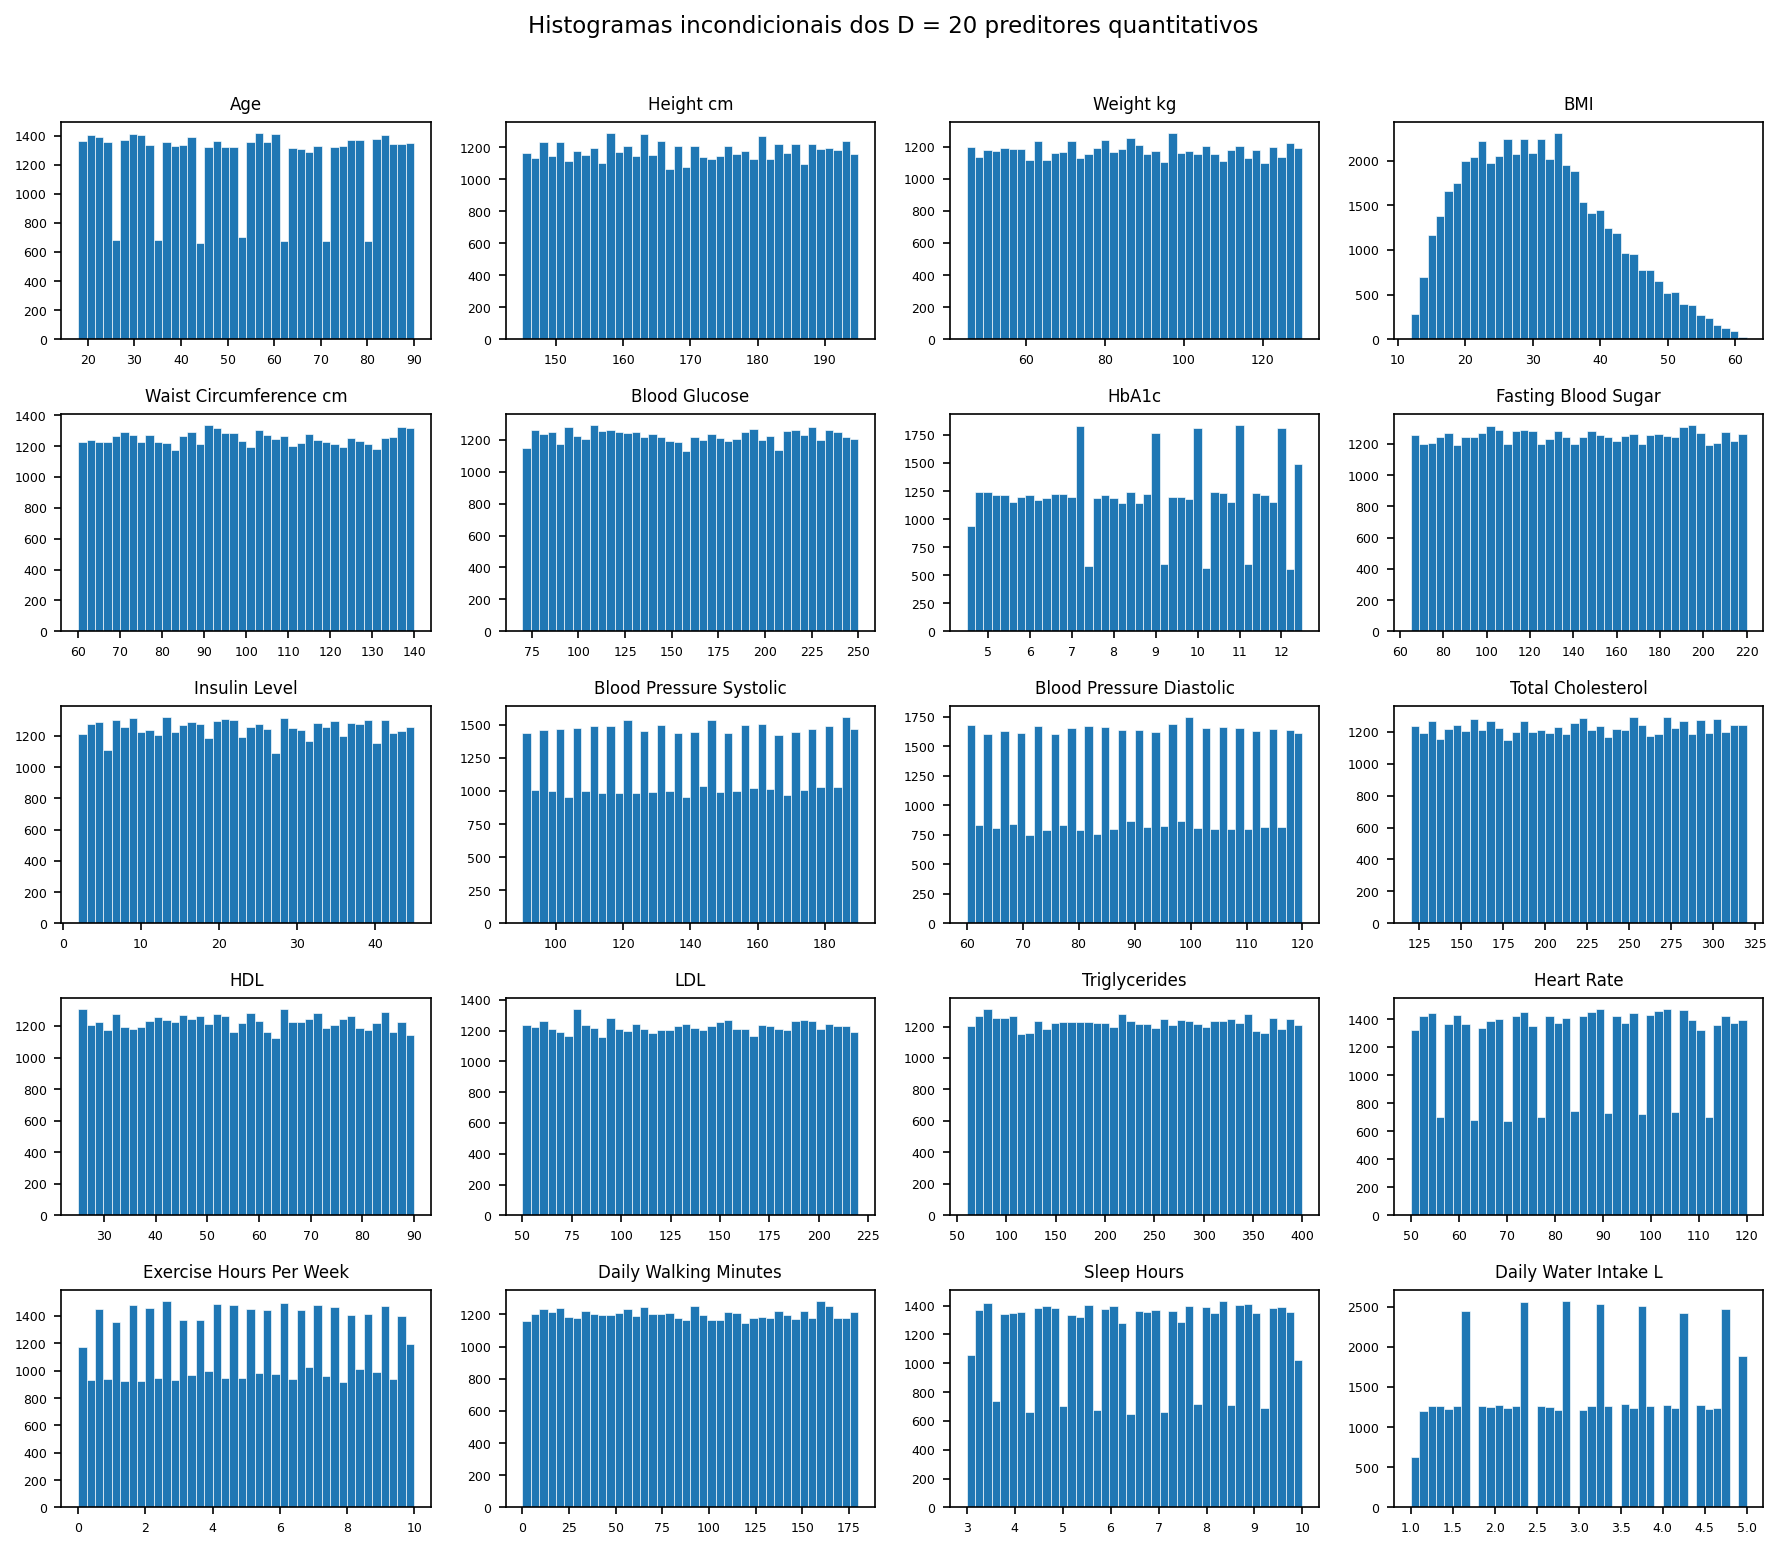
\includegraphics[width=\columnwidth]{histogramas_incondicionais.png}
\caption{Unconditional histograms of the 20 quantitative predictors.
All but the body mass index are visibly flat-topped.}
\label{fig:hist}
\end{figure}

% O achado: quase tudo e uniforme, nao gaussiano.
TODO: comentar que todas as assimetrias sao praticamente nulas, entre
$-0.015$ e $+0.008$, com a unica excecao do IMC ($\gamma = 0.432$).
Simetria, porem, nao implica normalidade, e e a curtose que resolve a
questao: 19 dos 20 preditores tem curtose excedente entre $-1.21$ e
$-1.19$, indistinguivel do valor $-6/5$ de uma distribuicao uniforme,
e os histogramas da Fig.~\ref{fig:hist} sao visivelmente achatados e
truncados. Os limites reforcam a leitura, pois sao numeros redondos
escolhidos por conveniencia e nao valores fisiologicos: idade de 18 a
90 anos, frequencia cardiaca de 50 a 120 bpm, triglicerideos de 60 a
400 mg/dL, sono de 3 a 10 horas.

TODO: a unica excecao e o IMC, com curtose $-0.45$ e assimetria
positiva, e a excecao tem explicacao mecanica: sendo o quociente
$\mathrm{peso}/\mathrm{altura}^2$ de duas uniformes independentes, ele
nao e uniforme. O IMC nao foi sorteado, foi \emph{calculado}. Este e o
primeiro dos tres sinais que convergem na Secao~\ref{subsec:pca}.

\subsection{Class-conditional analysis and discriminative power}
\label{subsec:cond}

% Bloco 2. O coracao do trabalho: algum preditor separa sozinho?
Table~\ref{tab:discrim} reports the class-conditional means and ranks
the predictors by the discriminative power of \eqref{eq:discrim};
Fig.~\ref{fig:histcond} shows the class-conditional histograms and
Fig.~\ref{fig:boxcond} the box-plots of the four strongest predictors.

\begin{table}[htbp]
\caption{Class-conditional means and discriminative power $\delta_d$,
predictors sorted by $\delta_d$}
\label{tab:discrim}
\centering
\begin{tabular}{lrrrr}
\toprule
Predictor & $\mu_{d|\mathrm{Low}}$ & $\mu_{d|\mathrm{Mod}}$
& $\mu_{d|\mathrm{High}}$ & $\delta_d$ \\
\midrule
Fasting Blood Sugar & 88.44 & 115.81 & 152.78 & 1.44 \\
HbA1c & 5.67 & 7.54 & 8.86 & 1.38 \\
Age & 38.81 & 46.89 & 56.53 & 0.84 \\
BMI & 25.60 & 28.31 & 31.92 & 0.61 \\
Weight kg & 75.68 & 81.77 & 89.61 & 0.57 \\
Blood Pressure Systolic & 127.98 & 134.73 & 142.25 & 0.49 \\
Total Cholesterol & 200.41 & 211.82 & 223.37 & 0.40 \\
Blood Pressure Diastolic & 85.55 & 88.06 & 90.80 & 0.30 \\
Height cm & 173.66 & 171.76 & 169.35 & 0.30 \\
Sleep Hours & 6.78 & 6.66 & 6.44 & 0.17 \\
HDL & 58.68 & 57.25 & 57.40 & 0.076 \\
Daily Water Intake L & 2.94 & 2.98 & 3.01 & 0.059 \\
Insulin Level & 23.05 & 23.61 & 23.44 & 0.045 \\
Waist Circumference cm & 100.85 & 100.08 & 99.91 & 0.041 \\
Daily Walking Minutes & 91.20 & 90.24 & 89.81 & 0.027 \\
Blood Glucose & 159.01 & 159.46 & 160.07 & 0.020 \\
Heart Rate & 85.36 & 85.10 & 85.13 & 0.013 \\
LDL & 135.04 & 135.35 & 134.90 & 0.009 \\
Exercise Hours Per Week & 5.03 & 5.02 & 5.02 & 0.006 \\
Triglycerides & 229.47 & 229.47 & 229.57 & 0.001
\\
\bottomrule
\end{tabular}
\end{table}

\begin{figure}[htbp]
\centering
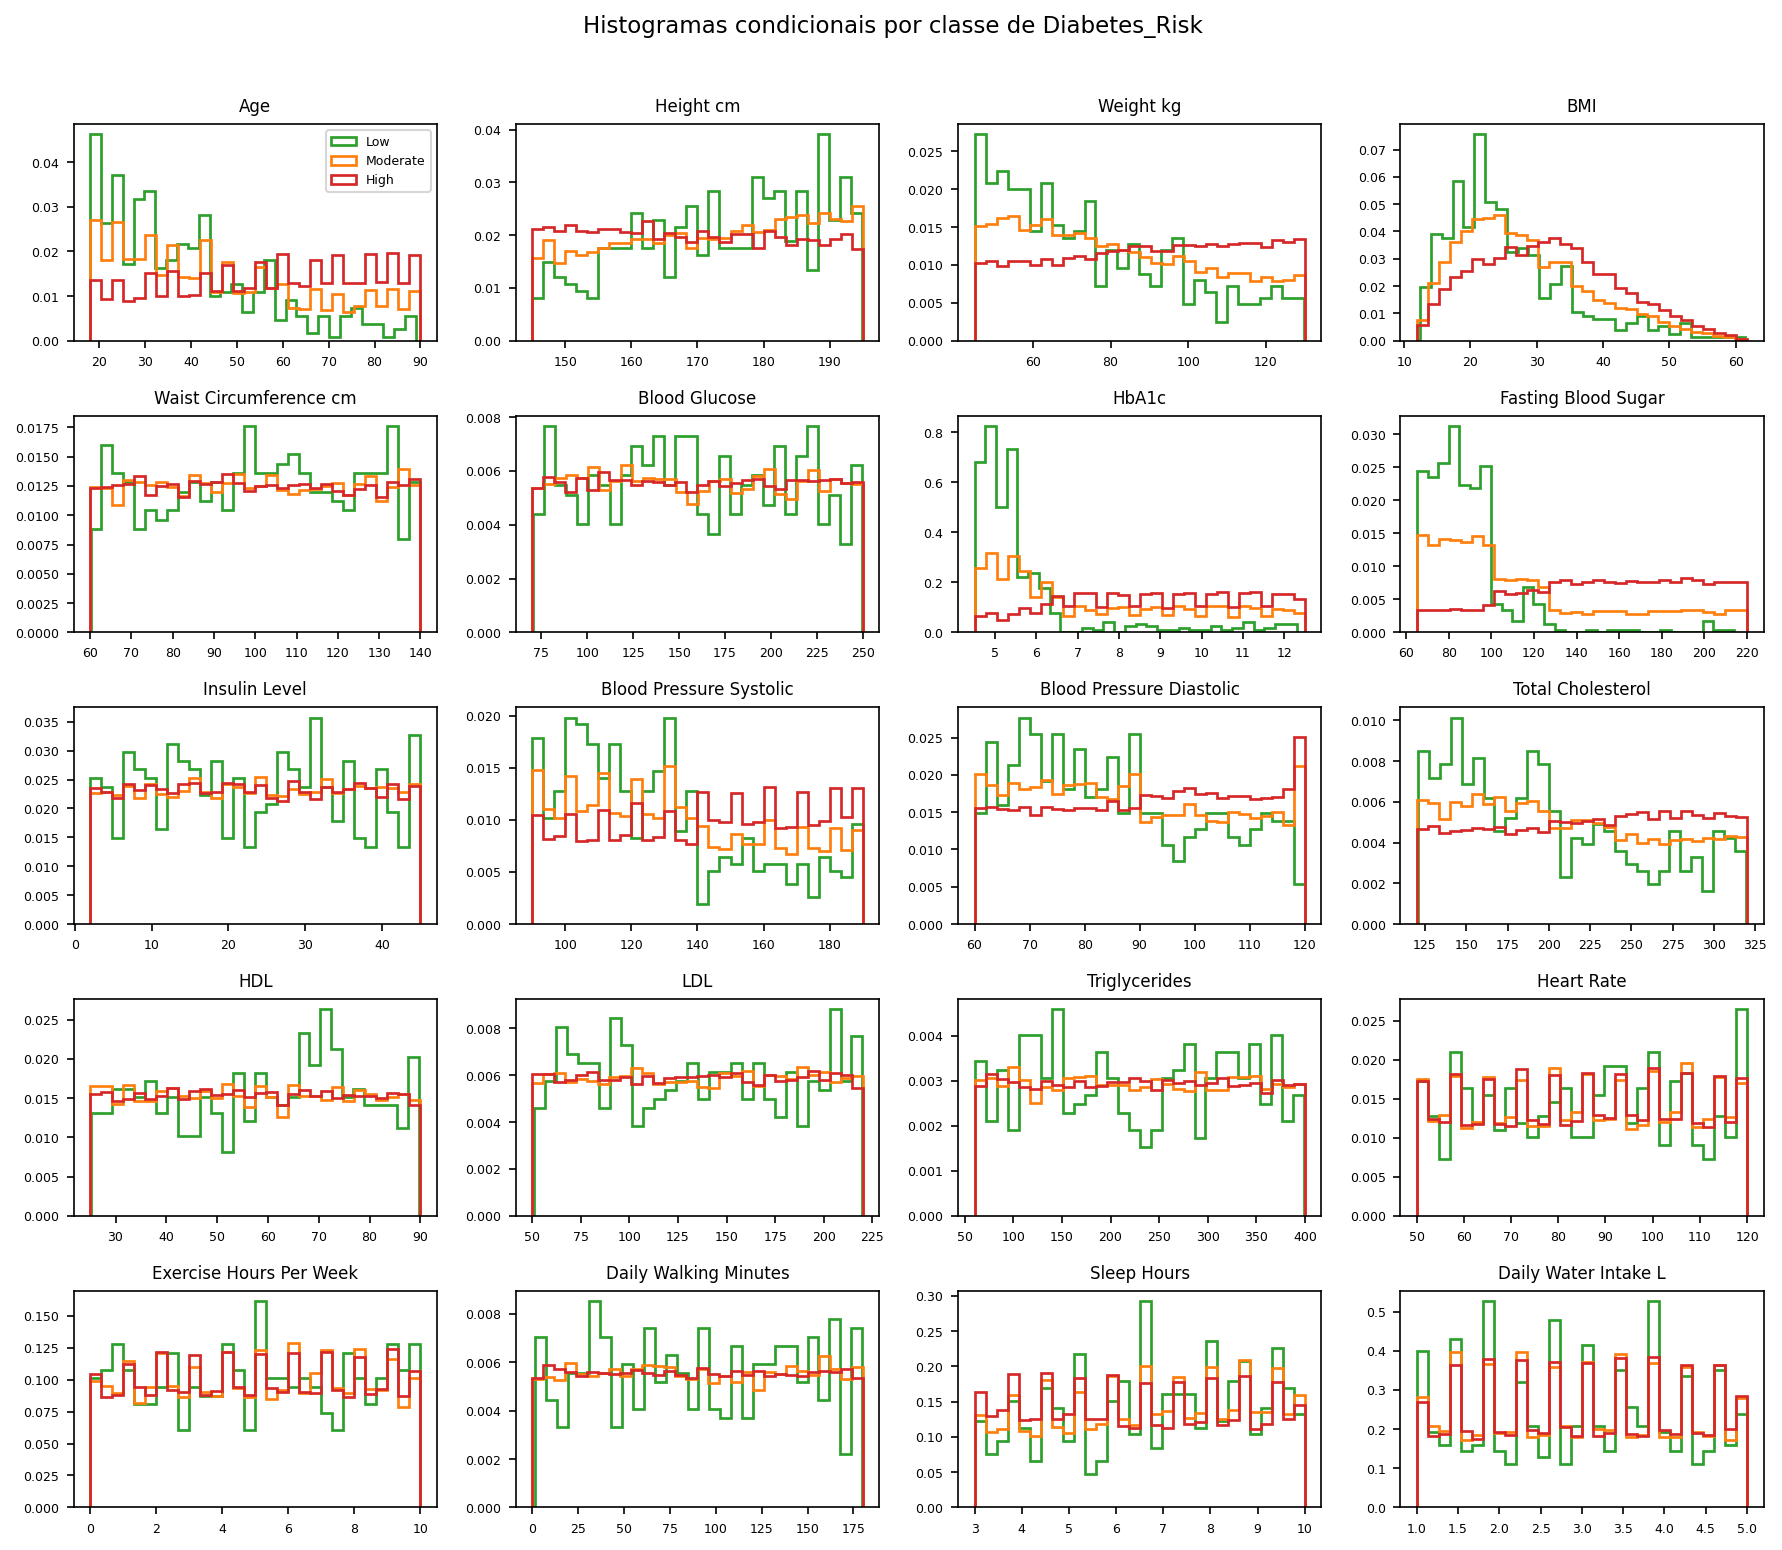
\includegraphics[width=\columnwidth]{histogramas_condicionais.png}
\caption{Class-conditional histograms of the 20 quantitative
predictors, normalised to unit area.}
\label{fig:histcond}
\end{figure}

\begin{figure}[htbp]
\centering
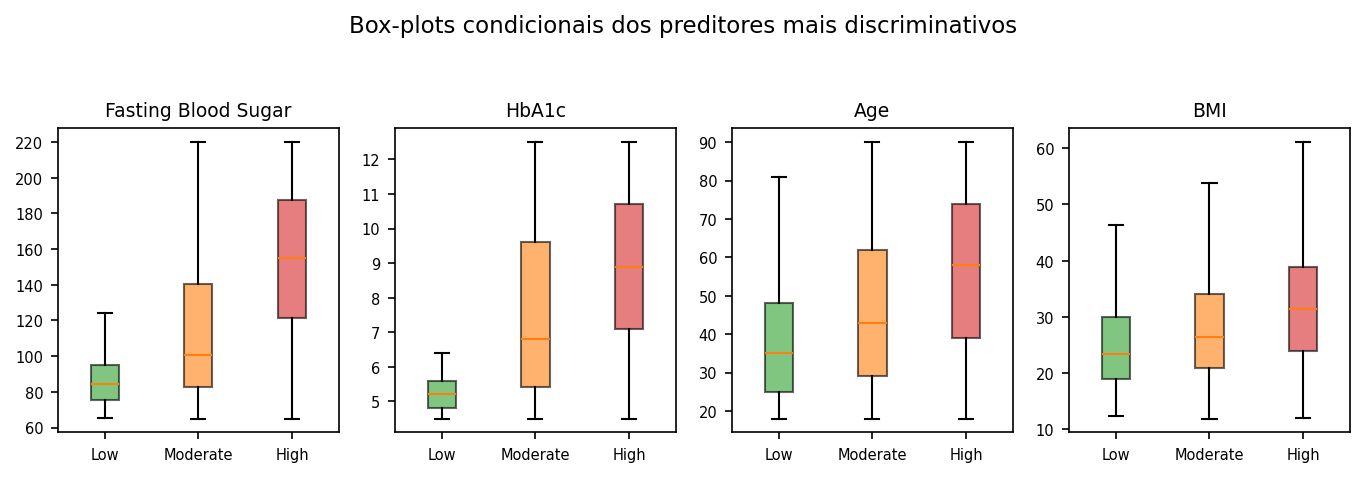
\includegraphics[width=\columnwidth]{boxplots_condicionais.png}
\caption{Class-conditional box-plots of the four most discriminative
predictors.}
\label{fig:boxcond}
\end{figure}

% A resposta direta a pergunta do enunciado.
TODO: responder diretamente a pergunta do enunciado. Sim, ha
preditores com poder discriminativo isolado, e sao dois: glicose em
jejum ($\delta = 1.44$) e HbA1c ($\delta = 1.38$), seguidos a
distancia por idade ($0.84$), IMC ($0.61$) e peso ($0.57$). Abaixo de
$\delta \approx 0.1$ os onze preditores restantes nao separam nada.

% Os numeros clinicos que valem citar.
TODO: HbA1c varia de $5.67$ (Low) a $8.86$ (High), exatamente a
travessia da faixa clinica de normal para diabetico \cite{ada2024};
glicose em jejum vai de $88.4$ a $152.8$~mg/dL, atravessando o limiar
diagnostico de 126; idade de $38.8$ a $56.5$ anos; IMC de $25.6$ a
$31.9$, isto e, de sobrepeso para obesidade. Nesse sentido, os
preditores que separam as classes sao clinicamente os corretos.

% As tres criticas. Isto e leitura critica, nao descricao: vale ponto.
Three observations qualify this apparent clinical fidelity.
TODO (i): a glicose casual tem $\delta = 0.020$, praticamente ruido,
enquanto a glicose em jejum tem $\delta = 1.44$. Clinicamente as duas
medem o mesmo substrato e caminham juntas, de modo que o gerador usou
uma e ignorou a outra.
TODO (ii): a circunferencia abdominal, marcador consagrado de risco
metabolico, tem $\delta = 0.041$ e ainda por cima \emph{decresce} com
o risco, de $100.85$ para $99.91$~cm.
TODO (iii): a altura decresce de $173.7$ para $169.4$~cm com
$\delta = 0.30$, o que nao e fisiologia mas consequencia algebrica de
o IMC dirigir o rotulo: a peso igual, quem e mais baixo tem IMC maior,
e portanto a altura herda um sinal invertido que ela nao possui na
populacao real.

\subsection{Bivariate analysis}
\label{subsec:bivar}

% Bloco 3. Matriz de correlacao + scatter matrix.
Fig.~\ref{fig:corr} shows the correlation matrix and
Fig.~\ref{fig:scatter} the pairwise scatter plots, coloured by class.

\begin{figure}[htbp]
\centering
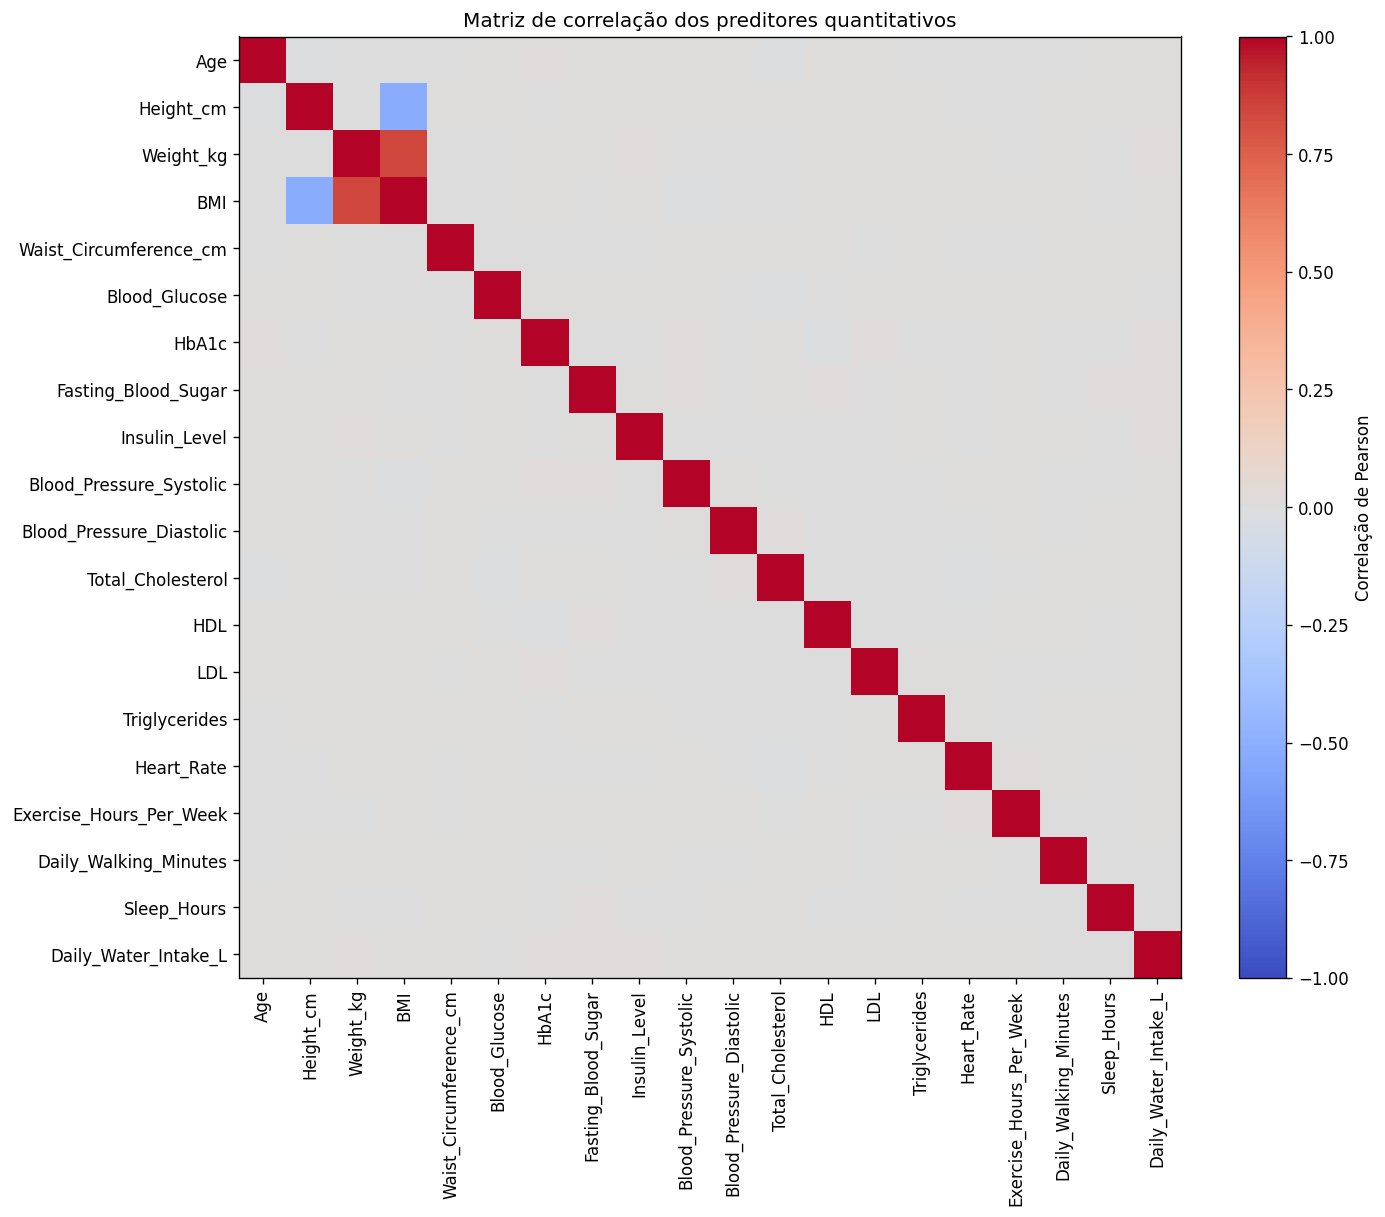
\includegraphics[width=\columnwidth]{matriz_correlacao.png}
\caption{Pairwise Pearson correlation matrix of the 20 quantitative
predictors.}
\label{fig:corr}
\end{figure}

\begin{figure}[htbp]
\centering
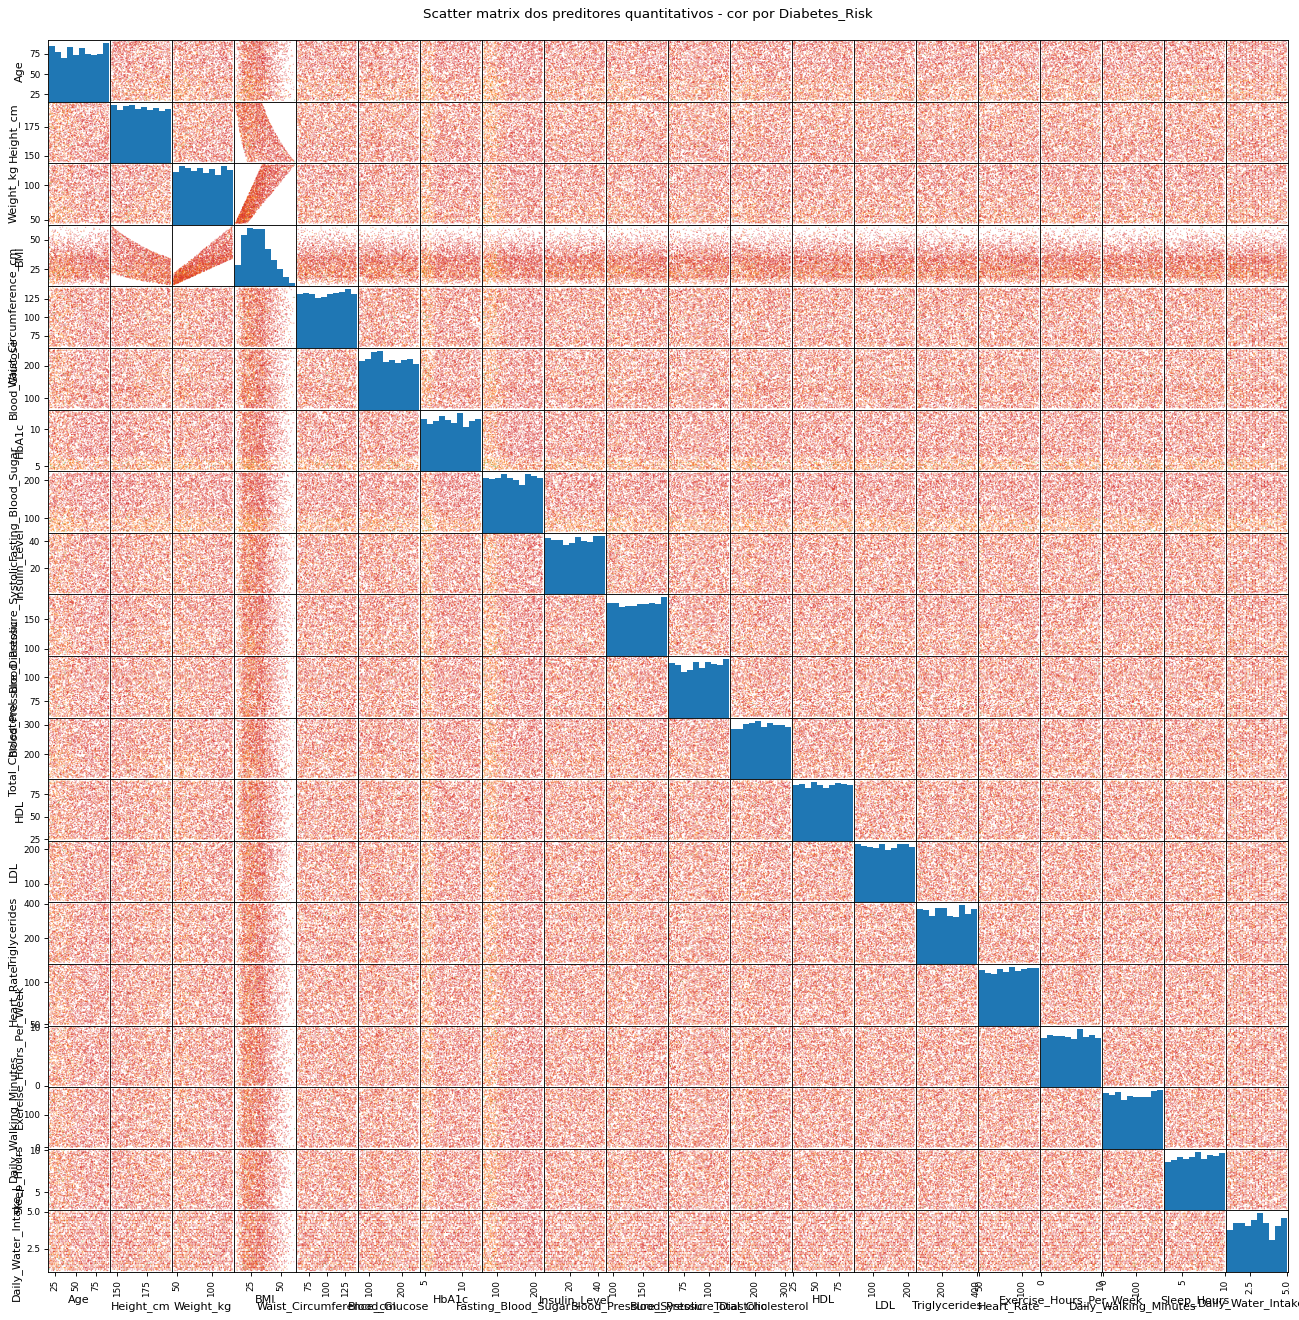
\includegraphics[width=\columnwidth]{scatter_matrix.png}
\caption{Pairwise scatter plots of the quantitative predictors on a
random subsample of 3{,}000 observations, coloured by risk class.}
\label{fig:scatter}
\end{figure}

% O segundo sinal: correlacoes nulas em quase todos os pares.
TODO: a matriz e essencialmente uma identidade. A mediana do modulo
das correlacoes fora da diagonal e $0.003$, e apenas dois pares fogem
disso: IMC com peso ($\rho = +0.843$) e IMC com altura
($\rho = -0.516$), que sao a propria definicao do indice e nao um
achado empirico. As nuvens da Fig.~\ref{fig:scatter} sao retangulos
sem estrutura, coerentes com preditores uniformes e independentes, e
nenhum par separa visualmente as classes.

% O achado mais interessante da secao.
TODO: o achado central e que HbA1c e glicose em jejum, os dois unicos
preditores com poder discriminativo relevante, tem $\rho = -0.005$
entre si. Num paciente real esses dois exames sao fortemente
correlacionados, pois a HbA1c integra a glicemia das semanas
anteriores. Aqui o rotulo depende dos dois por caminhos independentes,
o que e fisiologicamente impossivel e so se explica pelo processo
gerador. Este e o segundo sinal.

\subsection{Principal component analysis}
\label{subsec:pca}

% Bloco 4. O resultado mais forte, e ele e negativo. Tudo bem.
Table~\ref{tab:eigen} lists the eigenvalue spectrum and
Fig.~\ref{fig:pca} shows the projection onto the first two components.

\begin{table}[htbp]
\caption{Eigenvalue spectrum of the standardised covariance matrix
($20$ components, $33{,}689$ complete observations)}
\label{tab:eigen}
\centering
\begin{tabular}{lrrr}
\toprule
Component & $\lambda$ & Explained & Cumulative \\
\midrule
PC1 & 1.9943 & 9.97\% & 9.97\% \\
PC2 & 1.0371 & 5.19\% & 15.16\% \\
PC3 & 1.0327 & 5.16\% & 20.32\% \\
\midrule
PC4--PC19 & 0.9564--1.0292 & --- & --- \\
\midrule
PC20 & 0.0123 & 0.06\% & 100.00\%
\\
\bottomrule
\end{tabular}
\end{table}

\begin{figure}[htbp]
\centering
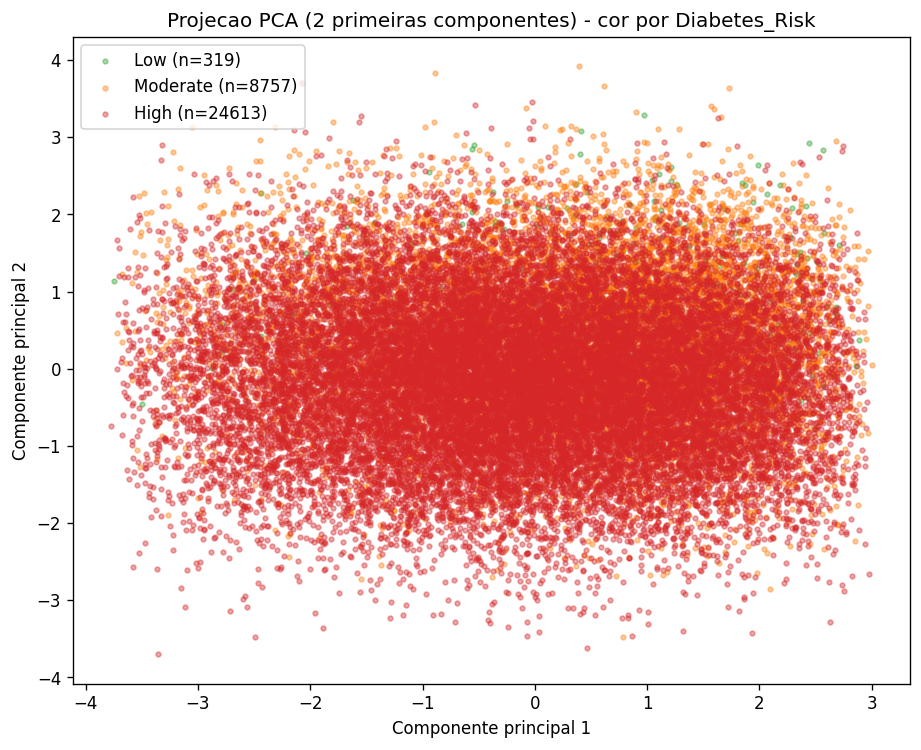
\includegraphics[width=\columnwidth]{pca_projecao.png}
\caption{Observations projected onto the first two principal
components, coloured by risk class.}
\label{fig:pca}
\end{figure}

% A assinatura dos autovalores: terceiro sinal, vindo de um terceiro
% metodo.
TODO: apos a padronizacao a soma dos autovalores e 20, de modo que um
conjunto de preditores mutuamente nao correlacionados produz vinte
autovalores iguais a $1$. E quase exatamente o que se observa: as
componentes PC2 a PC19 ficam entre $0.956$ e $1.037$, uma faixa de
menos de $\pm 4\%$ em torno da unidade. Um espectro plano e a
assinatura da ausencia de estrutura linear, e constitui o terceiro
sinal independente, vindo de um terceiro metodo, do que a curtose e a
matriz de correlacao ja indicavam.

% As duas excecoes sao a mesma coisa: a identidade do IMC.
TODO: as duas excecoes sao a mesma coisa vista por dois lados. Os
\emph{loadings} da primeira componente ($\lambda = 1.994$) sao IMC
$-0.706$, peso $-0.602$ e altura $+0.372$, com todos os demais abaixo
de $0.02$ em modulo; os da ultima ($\lambda = 0.0123$) sao IMC
$+0.708$, peso $-0.603$ e altura $+0.368$. O PCA isolou sozinho a
identidade $\mathrm{IMC} = \mathrm{peso}/\mathrm{altura}^2$: a maior
variancia esta no plano gerado por essas tres variaveis, e o autovalor
quase nulo mede a dependencia quase deterministica entre elas, quase e
nao exatamente porque a relacao e nao linear e o PCA so captura sua
melhor aproximacao linear. Esta e a unica relacao estrutural presente
no conjunto, e o metodo a encontrou sem ser instruido.

% Responder LITERALMENTE as tres perguntas do enunciado.
TODO: responder as tres perguntas do item 5. (i) As classes nao ficam
bem separadas na projecao, e ficam \emph{pior} separadas do que na
analise monovariada de HbA1c ou glicose em jejum. (ii) Nao ha
fronteira linear visivel. (iii) \emph{Moderate} se sobrepoe
fortemente a \emph{High}, e \emph{Low} e praticamente invisivel, tanto
por conter apenas 470 pontos quanto por ocupar a mesma regiao que as
outras duas.

% Paragrafo de fechamento: a tensao entre os dois achados.
TODO: fechar com a tensao aparente. As duas primeiras componentes
explicam apenas $15.2\%$ da variancia e a projecao nao separa nada,
enquanto a analise monovariada encontrou sinal forte e clinicamente
coerente. As duas coisas sao verdadeiras ao mesmo tempo porque medem
objetos diferentes: o PCA maximiza variancia, nao separabilidade, e
quando os preditores sao quase todos independentes nao existe direcao
de alta variancia onde a informacao de classe se concentre. Alem
disso, a unica direcao de variancia elevada que o conjunto possui, a
do IMC, e justamente uma relacao algebrica sem conteudo discriminativo
proprio. O PCA nao falhou; ele reportou corretamente que nao ha
estrutura multivariada a reportar.

% =====================================================================
% IV. CONCLUSION
% =====================================================================
\section{Conclusion}
\label{sec:conclusion}

TODO: os tres achados convergem para uma leitura unica. A curtose
uniforme em 19 de 20 preditores, a mediana de $0.003$ nas correlacoes
e o espectro de autovalores plano sao tres medidas independentes do
mesmo fato: os preditores foram amostrados de distribuicoes uniformes
independentes em intervalos redondos, e o rotulo foi atribuido a
posteriori em funcao de poucas variaveis, principalmente glicose em
jejum, HbA1c, idade e IMC. A unica dependencia presente e algebrica,
nao fisiologica.

TODO: a implicacao pratica. Um dataset assim serve para exercitar o
fluxo de analise, que e o objetivo deste trabalho, mas nao suporta
conclusoes clinicas nem permite avaliar de forma realista metodos
multivariados, justamente porque a estrutura multivariada que esses
metodos existem para explorar foi eliminada na geracao. Um
classificador treinado aqui alcancaria bom desempenho aparente usando
dois preditores, e esse resultado nao transferiria para dados reais.
Registrar isso e, em si, um resultado da analise exploratoria.

% =====================================================================
% REFERENCES -- minimo 5 ou 6.
% =====================================================================
\bibliographystyle{IEEEtran}
\bibliography{refs}

\end{document}
